
\documentclass[10pt,letterpaper]{article}

\usepackage[letterpaper,margin=0.70in,headheight=22pt,headsep=16pt,footskip=24pt]{geometry}
\usepackage[T1]{fontenc}
\usepackage[utf8]{inputenc}
\usepackage{lmodern}
\usepackage{microtype}
\usepackage{xcolor}
\usepackage{graphicx}
\usepackage{booktabs}
\usepackage{array}
\usepackage{tabularx}
\usepackage{longtable}
\usepackage{amsmath,amssymb}
\usepackage{tikz}
\usetikzlibrary{arrows.meta,positioning,calc,shapes.geometric,decorations.pathreplacing,fit}
\usepackage{enumitem}
\usepackage{fancyhdr}
\usepackage{titlesec}
\usepackage{caption}
\usepackage{listings}
\usepackage{xurl}
\usepackage[hidelinks]{hyperref}
\usepackage{lastpage}
\usepackage{float}
\usepackage{placeins}

\definecolor{FStatRed}{HTML}{A00000}
\definecolor{FStatGray}{HTML}{555555}
\definecolor{FStatBlue}{HTML}{144E8C}
\definecolor{LightGray}{HTML}{F3F3F3}
\definecolor{MidGray}{HTML}{D9D9D9}
\definecolor{DarkText}{HTML}{1A1A1A}
\definecolor{GoodGreen}{HTML}{2B7A2B}
\definecolor{WarnOrange}{HTML}{A65E00}

\renewcommand{\familydefault}{\sfdefault}
\setlength{\parindent}{0pt}
\setlength{\parskip}{5pt}
\renewcommand{\arraystretch}{1.15}
\sloppy
\setlist[itemize]{leftmargin=1.2em,itemsep=2pt,topsep=2pt}
\setlist[enumerate]{leftmargin=1.4em,itemsep=2pt,topsep=2pt}

\titleformat{\section}{\Large\bfseries\color{DarkText}}{}{0pt}{}[\vspace{-3pt}\color{FStatRed}\titlerule]
\titleformat{\subsection}{\large\bfseries\color{DarkText}}{}{0pt}{}
\titleformat{\subsubsection}{\normalsize\bfseries\color{DarkText}}{}{0pt}{}

\newcommand{\code}[1]{\texttt{\detokenize{#1}}}
\newcommand{\apicode}[1]{\texttt{\detokenize{#1}}}
\newcommand{\yes}{\textcolor{GoodGreen}{Yes}}
\newcommand{\no}{\textcolor{FStatGray}{No}}
\newcolumntype{Y}{>{\raggedright\arraybackslash}X}
\newcolumntype{L}[1]{>{\raggedright\arraybackslash}p{#1}}
\newcolumntype{C}[1]{>{\centering\arraybackslash}p{#1}}
\captionsetup{font=small,labelfont=bf}

\lstdefinestyle{shell}{
  basicstyle=\ttfamily\footnotesize,
  breaklines=true,
  columns=fullflexible,
  frame=single,
  rulecolor=\color{MidGray},
  backgroundcolor=\color{LightGray},
  keepspaces=true,
  showstringspaces=false
}
\lstdefinestyle{cstyle}{
  basicstyle=\ttfamily\footnotesize,
  breaklines=true,
  columns=fullflexible,
  frame=single,
  rulecolor=\color{MidGray},
  backgroundcolor=\color{LightGray},
  keepspaces=true,
  showstringspaces=false
}
\lstset{style=shell}

\newcommand{\notebox}[1]{%
  \vspace{4pt}\noindent\fcolorbox{FStatBlue}{LightGray}{%
  \begin{minipage}{0.965\linewidth}%
  \textbf{Note:} #1%
  \end{minipage}}\vspace{4pt}}

\newcommand{\importantbox}[1]{%
  \vspace{4pt}\noindent\fcolorbox{FStatRed}{LightGray}{%
  \begin{minipage}{0.965\linewidth}%
  \textbf{Important:} #1%
  \end{minipage}}\vspace{4pt}}

\newcommand{\field}[1]{\texttt{\detokenize{#1}}}
\newcommand{\dB}{\,\mathrm{dB}}


\pagestyle{fancy}
\fancyhf{}
\fancyhead[L]{\small PilotProxy-UG001}
\fancyhead[C]{\small CUDA F-Statistic DTV Pilot Detector v0.1.0}
\fancyhead[R]{\small User Guide}
\fancyfoot[L]{\small PilotProxy-UG001 v1.4}
\fancyfoot[C]{\small Standalone ATSC 1.0 pilot-tone detector}
\fancyfoot[R]{\small Page \thepage\ of \pageref{LastPage}}
\renewcommand{\headrulewidth}{0.8pt}
\renewcommand{\headrule}{\hbox to\headwidth{\color{FStatRed}\leaders\hrule height \headrulewidth\hfill}}
\renewcommand{\footrulewidth}{0.8pt}
\renewcommand{\footrule}{\hbox to\headwidth{\color{FStatRed}\leaders\hrule height \footrulewidth\hfill}}

\title{PilotProxy CUDA F-Statistic DTV Pilot Detector v0.1.0\\User Guide}
\author{West Virginia University}
\date{PilotProxy-UG001 v1.4 \\ July 2, 2026}

\begin{document}
\thispagestyle{empty}
\begin{tikzpicture}[remember picture,overlay]
  \draw[FStatRed,line width=2pt] ($(current page.north west)+(0.72in,-0.35in)$) -- ($(current page.north east)+(-0.72in,-0.35in)$);
  \draw[FStatRed,line width=1pt] ($(current page.south west)+(0.72in,0.45in)$) -- ($(current page.south east)+(-0.72in,0.45in)$);
\end{tikzpicture}
\vspace*{0.25in}
{\fontsize{30}{32}\selectfont\bfseries\color{FStatRed}PilotProxy}\par
\vspace{0.12in}
{\fontsize{23}{26}\selectfont\bfseries CUDA F-Statistic DTV Pilot Detector v0.1.0}\par
\vspace{0.08in}
{\Large User Guide}\par
\vspace{0.35in}
{\large PilotProxy-UG001 v1.4}\par
{\large July 2, 2026}\par
\vfill
\begin{tabularx}{\linewidth}{|>{\bfseries}L{0.25\linewidth}|Y|}
\hline
Document scope & Source-tree use, CUDA build, ATSC waveform generation, validation, detection, and interpretation of fixed-point kernel outputs.\\ \hline
Package version & \code{pilot-proxy} v0.1.0.\\ \hline
Primary runtime controls & Target channel or pilot frequency selects weights; the detector runtime controls are frame size and DTV data-shelf SNR threshold.\\ \hline
CHIME/CANFAR mode & The standalone synthetic detector supports thresholded operation; the CHIME real-data workflow uses parameter-free, norm-corrected positive-excess masking ($F>\mu_0$).\\ \hline
Project affiliation & West Virginia University.\\ \hline
\end{tabularx}
\newpage

\section*{Revision History}
\begin{tabularx}{\linewidth}{|L{0.18\linewidth}|L{0.14\linewidth}|Y|}
\hline
\textbf{Date} & \textbf{Version} & \textbf{Revision}\\ \hline
July 2, 2026 & 1.4 & Norm-corrected positive-excess mask ($F>\mu_0$, exact integer form); LaTeX-styled figures with vector-PDF export; publication-analysis commands (\code{inject-pilot-tone}, \code{analyze-injection-recovery}, \code{analyze-cleaning-tradeoff}).\\ \hline
May 29, 2026 & 1.3 & Added receiver-profile integration workflow, full stream-map example, and profile-driven weight generation.\\ \hline
May 29, 2026 & 1.2 & Regenerated for standalone \code{pilot-proxy} v0.1.0.  Added release-candidate CLI names, physical-channel support, strict JSON reporting, calibration field names, and channel-21 edge-wrap handling.\\ \hline
May 29, 2026 & 1.1 & Standalone DTV user guide.  Instrument-specific content removed.\\ \hline
May 29, 2026 & 1.0 & Initial CUDA F-statistic kernel user guide.\\ \hline
\end{tabularx}
\newpage

\tableofcontents
\newpage

\section{Introduction}

PilotProxy is a standalone CUDA F-statistic detector and GNU Radio ATSC 1.0 testbench.  It estimates and detects sub-noise-floor DTV signals by using the ATSC pilot tone as a proxy for the underlying DTV data shelf.

The package does one thing: given a local ATSC pilot peak measured by the F-statistic, estimate the equivalent ATSC 1.0 data-shelf SNR relative to the non-DTV noise floor.  It does not require external receiver data products, instrument-specific metadata, or deployment-specific masking workflows.

\subsection{Detector Objective}

\begin{quote}
Given a local ATSC pilot peak measured by the F-statistic, estimate the equivalent sub-noise-floor ATSC 1.0 data-shelf SNR relative to the non-DTV noise floor.
\end{quote}

This guide describes how to build the kernel, generate and audit a GNU Radio ATSC waveform, add noise at a requested shelf SNR, quantize into the locked packed-int4 detector format, run the CUDA kernel, and interpret the results.

\subsection{Package Contents}

\begin{longtable}{|L{0.30\linewidth}|L{0.62\linewidth}|}
\hline
\textbf{Path} & \textbf{Contents}\\ \hline
\code{cuda/} & CUDA kernel, public C header, CPU reference model, and C/CUDA tests.\\ \hline
\code{src/pilot_proxy/} & Python package for kernel loading, detector geometry, reference channelization, DTV unit conversion, channel helpers, and detection.\\ \hline
\code{src/pilot_proxy/testbench/} & GNU Radio ATSC generation, waveform audit, AWGN injection, quantization, and SNR evaluation.\\ \hline
\code{weights/} & Prebuilt ATSC reference detector weights for channels 14-36.\\ \hline
\code{docs/} & Markdown definitions, data sheet, and user guide source.\\ \hline
\code{examples/quickstart.sh} & End-to-end release sanity-check workflow.\\ \hline
\end{longtable}

\section{Definitions}

The CUDA detector reports the raw F-statistic:
\begin{equation}
  F=\frac{2P_t}{P_{r1}+P_{r2}},\qquad \rho=F-1.
\end{equation}
The quantity \(10\log_{10}F\) is the F-statistic level.  It is not the physical pilot-to-noise ratio, because \(F=1\) means no pilot excess.

The one-bin pilot-excess PNR is:
\begin{equation}
  \mathrm{PNR}_{\mathrm{bin},dB}=10\log_{10}(F-1).
\end{equation}
The DTV data-shelf SNR estimate is:
\begin{equation}
  \mathrm{SNR}_{\mathrm{shelf},dB} = \mathrm{PNR}_{\mathrm{bin},dB}
  -10\log_{10}(B_{\mathrm{DTV}}/B_{\mathrm{bin}})
  +\mathrm{pilot\_below\_data\_db}
  -10\log_{10}(\eta_p).
\end{equation}
The default geometry gives:
\begin{equation}
  B_{\mathrm{bin}}=\frac{400\,\mathrm{MHz}}{1024\times128}=3051.7578125\,\mathrm{Hz},
\end{equation}
so:
\begin{equation}
  10\log_{10}(6\,\mathrm{MHz}/B_{\mathrm{bin}})=32.936\dB.
\end{equation}

\notebox{A 1 dB F-statistic level means \(F=1.2589\), \(\rho=0.2589\), \(\mathrm{PNR}_{\mathrm{bin}}=-5.868\dB\), and \(\mathrm{SNR}_{\mathrm{shelf}}\approx -27.50\dB\) for the default 3.052 kHz detector bin.}


\begin{figure}[H]
\centering
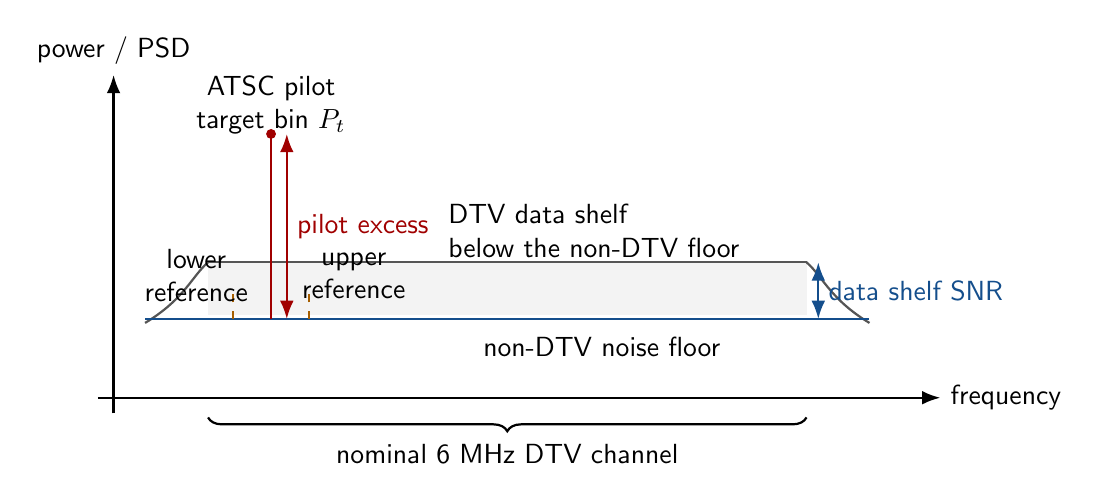
\begin{tikzpicture}[x=1.0cm,y=1.0cm,>=Latex]
  \draw[->,thick] (-0.2,0) -- (10.5,0) node[right]{frequency};
  \draw[->,thick] (0,-0.2) -- (0,4.1) node[above]{power / PSD};
  \draw[fill=LightGray,draw=none] (1.2,1.05) rectangle (8.8,1.72);
  \draw[thick,FStatGray] (1.2,1.72) -- (8.8,1.72);
  \draw[thick,FStatGray] (0.4,0.95) .. controls (0.9,1.25) and (1.0,1.55) .. (1.2,1.72);
  \draw[thick,FStatGray] (8.8,1.72) .. controls (9.0,1.55) and (9.1,1.25) .. (9.6,0.95);
  \draw[thick,FStatBlue] (0.4,1.0) -- (9.6,1.0);
  \draw[thick,FStatRed] (2.0,1.0) -- (2.0,3.35);
  \draw[fill=FStatRed,draw=FStatRed] (2.0,3.35) circle (0.055);
  \draw[dashed,thick,WarnOrange] (1.52,1.0) -- (1.52,1.35);
  \draw[dashed,thick,WarnOrange] (2.48,1.0) -- (2.48,1.35);
  \draw[<->,thick,FStatRed] (2.20,1.0) -- (2.20,3.35) node[midway,right]{pilot excess};
  \draw[<->,thick,FStatBlue] (8.95,1.0) -- (8.95,1.72) node[midway,right]{data shelf SNR};
  \draw[decorate,decoration={brace,mirror,amplitude=5pt},thick] (1.2,-0.25) -- (8.8,-0.25)
    node[midway,below=6pt]{nominal 6 MHz DTV channel};
  \node[align=center] at (2.0,3.72) {ATSC pilot\\target bin $P_t$};
  \node[align=center] at (1.05,1.55) {lower\\reference};
  \node[align=center] at (3.05,1.55) {upper\\reference};
  \node[align=left] at (6.1,2.12) {DTV data shelf\\below the non-DTV floor};
  \node[align=left] at (6.2,0.65) {non-DTV noise floor};
\end{tikzpicture}
\caption{Definitions used by the standalone detector.  The kernel measures the target pilot-bin power relative to local reference bins.  Host software converts the one-bin pilot-excess measurement to a 6 MHz-equivalent DTV data-shelf SNR.}
\label{fig:spectrum_definitions}
\end{figure}


\section{Installation Model}

This v0.1.0 release is intended to run from a cloned source tree.  Use:
\begin{lstlisting}[style=shell]
PYTHONPATH=src python -m pilot_proxy.cli --help
\end{lstlisting}
Editable installs are supported:
\begin{lstlisting}[style=shell]
python -m pip install -e .
\end{lstlisting}
A wheel-style install with packaged CUDA and weight resources is not the primary supported mode for v0.1.0.

\subsection{Python Environments}

Use two Python interpreters when GNU Radio is installed as a system package:
\begin{itemize}
  \item GNU Radio Python: used for ATSC generation and GNU Radio AWGN, typically \code{/usr/bin/python3}.
  \item CUDA Python: used for CuPy, the CUDA shared library, and detector evaluation, typically a conda environment with \code{numpy}, \code{pytest}, and \code{cupy-cuda12x}.
\end{itemize}

On WSL, keep the two environments separate:
\begin{lstlisting}[style=shell]
GNURADIO_PYTHON=/usr/bin/python3
CUDA_PYTHON=$HOME/miniconda3/envs/fstat/bin/python
CUDA_LD_LIBRARY_PATH=/usr/lib/wsl/lib
\end{lstlisting}

On WSL, do not add the conda environment \code{lib/} directory to
\code{LD_LIBRARY_PATH}.  It can make \code{/usr/bin/bash} load conda's
\code{libtinfo.so.6} and print a \code{no version information available}
warning.  The CUDA detector examples only require the WSL CUDA driver path.
Use \code{PYTHONNOUSERSITE=1} when invoking GNU Radio Python so that user-site packages do not shadow the NumPy build used by GNU Radio.

\section{Build and Test}

\subsection{Build the CUDA Kernel}

Build for the target GPU architecture:
\begin{lstlisting}[style=shell]
make build-kernel SM=89
\end{lstlisting}
This builds \code{cuda/libfstatistic.so} and stages a copy to:
\begin{lstlisting}[style=shell]
~/.cache/pilot_proxy/libfstatistic.so
\end{lstlisting}
On WSL, the cached copy avoids loading the shared library directly from \code{/mnt/c}.  If you rebuild only under \code{cuda/}, remove the staged copy with:
\begin{lstlisting}[style=shell]
make clean-cache
\end{lstlisting}

\subsection{Run Tests}

Run Python tests:
\begin{lstlisting}[style=shell]
PYTHONPATH=src python -m pytest tests -q
\end{lstlisting}
Run CUDA/kernel tests on a CUDA-capable host:
\begin{lstlisting}[style=shell]
make -C cuda test SM=89 DP4A=1
\end{lstlisting}
The release-candidate source tree used for this document passed the Python release checks available in this environment.  Run CUDA and GNU Radio quickstart tests on the target machine before tagging a release.

\section{Quickstart}

The provided script performs the release sanity-check flow:
\begin{lstlisting}[style=shell]
SM=89 bash examples/quickstart.sh
\end{lstlisting}
The expected output includes a waveform audit, detector input generation, SNR evaluation, and detection JSON.  A typical excerpt is:
\begin{lstlisting}[style=shell]
measured_pilot_frequency_hz=-2690559.44
measured_pilot_to_data_power_db=-11.9
measured_pilot_below_data_db=11.9
requested_snr_shelf_db, measured_truth_snr_shelf_db, fstat_raw, fstat_level_db, pnr_bin_db, estimated_snr_shelf_db, snr_error_db
 -26.000,  -26.005,   1.436541,    1.541,   -3.967,  -25.603,    0.402
blocks, masks_set, threshold_snr_shelf_db, threshold_pnr_bin_db, threshold_fstat_raw, threshold_half_num, threshold_half_den, rational_overflow_count
1, 1, -26.000, -4.364, 1.36610123, 2254618387, 3300807204, 0
\end{lstlisting}

\section{Generate and Audit an ATSC Waveform}

\subsection{Generate a Clean ATSC Signal}

Run ATSC generation with GNU Radio Python:
\begin{lstlisting}[style=shell]
PYTHONNOUSERSITE=1 PYTHONPATH=src /usr/bin/python3 \
  -m pilot_proxy.testbench.generate_atsc_signal \
  --output-iq generated/atsc/atsc_8vsb_complex64.cfile \
  --num-iq-samples 600000
\end{lstlisting}

\subsection{Audit the Clean Waveform}

Run the audit before detector evaluation:
\begin{lstlisting}[style=shell]
PYTHONPATH=src "$HOME/miniconda3/envs/fstat/bin/python" \
  -m pilot_proxy.testbench.audit_atsc_signal \
  --input-iq generated/atsc/atsc_8vsb_complex64.cfile
\end{lstlisting}
The audit records pilot frequency, pilot/data power, occupied bandwidth, shelf flatness, and edge rolloff metrics.  The field \field{measured_pilot_to_data_power_db} is signed \(10\log_{10}(P_{\mathrm{pilot}}/P_{\mathrm{data}})\).  The field \field{measured_pilot_below_data_db} is the positive magnitude.

\notebox{The audit reports pilot frequency in the generated complex-baseband coordinate.  For physical channel 14, the baseband pilot corresponds to an RF pilot at 470.309441 MHz after reference-band placement.}

\section{Reference Channelizer and Detector Resolution}

The standalone reference front end is a neutral PFB/channelizer model:
\begin{longtable}{|L{0.36\linewidth}|L{0.56\linewidth}|}
\hline
\textbf{Quantity} & \textbf{Value}\\ \hline
Real ADC sample rate & 800 MS/s \\ \hline
Reference lower band edge & 400 MHz \\ \hline
Reference bandwidth & 400 MHz \\ \hline
PFB taps & 4 \\ \hline
PFB FFT size & 2048 real-input samples \\ \hline
Usable positive-frequency channels & 1024 \\ \hline
Coarse-channel spacing & 390.625 kHz \\ \hline
Detector window & 128 samples \\ \hline
Fine detector-bin width & 3051.7578125 Hz \\ \hline
\end{longtable}
The fine detector-bin width is used in the default PNR-to-shelf-SNR conversion.

\section{Channel Selection}

List physical channels supported by the shipped weight bank:
\begin{lstlisting}[style=shell]
PYTHONPATH=src python -m pilot_proxy.cli list-channels
\end{lstlisting}
The included weights cover physical channels 14 through 36.  ATSC helper routines can compute UHF channel frequencies outside that range, but detection requires a matching manifest-backed weight row.

The default channel is physical channel 14:
\begin{equation}
  f_{\mathrm{lower}}=470\,\mathrm{MHz},\quad f_{\mathrm{pilot}}=470.309441\,\mathrm{MHz},\quad f_{\mathrm{center}}=473\,\mathrm{MHz}.
\end{equation}
Physical channel 21 is a reference-boundary case.  Its selected weight layout preserves the requested \(-2,+2\) reference offsets by wrapping the lower reference across the circular coarse-channel spectrum and reports \field{adaptive_reference_placement=true}.

\section{Quantize and Create Detector Input}

Create a packed detector matrix:
\begin{lstlisting}[style=shell]
PYTHONPATH=src "$HOME/miniconda3/envs/fstat/bin/python" \
  -m pilot_proxy.testbench.quantize \
  --input-iq generated/atsc/atsc_8vsb_complex64.cfile \
  --physical-channel 14 \
  --frame-size-samples 16384
\end{lstlisting}
The output matrix is row-major and has shape \code{(rows, 128)} or \code{(batch, rows, 128)}.  The dtype must be \code{int8}.  The CUDA path validates dtype and shape before handing pointers to the kernel.

\section{Evaluate Shelf-SNR Recovery}

Run the end-to-end validation evaluator with CUDA/CuPy Python:
\begin{lstlisting}[style=shell]
LD_LIBRARY_PATH=/usr/lib/wsl/lib \
PYTHONPATH=src "$HOME/miniconda3/envs/fstat/bin/python" \
  -m pilot_proxy.testbench.evaluate_snr \
  --input-iq generated/atsc/atsc_8vsb_complex64.cfile \
  --physical-channel 14 \
  --frame-size-samples 16384 \
  --requested-snr-shelf-db -26 \
  --threshold-snr-shelf-db -26 \
  --noise-trials 10 \
  --noise-source gnuradio \
  --gnuradio-python /usr/bin/python3
\end{lstlisting}
Outputs are written under \code{generated/dtv_snr_eval/}:
\begin{itemize}
  \item \code{dtv_snr_eval.csv}: per-trial validation rows;
  \item \code{dtv_snr_summary.csv}: grouped summary;
  \item \code{dtv_snr_eval.json}: full strict-JSON validation report.
\end{itemize}

If no explicit \code{--requested-snr-shelf-db} values or
\code{--snr-start-db}/\code{--snr-stop-db}/\code{--snr-step-db} range is
provided, the evaluator runs the public sweep from \(-60\dB\) to \(0\dB\) in
3 dB steps.  One \code{--noise-trials} count corresponds to one independent
detector frame at each requested SNR and frequency offset.  For a smoother 3 dB
sweep plot, use several frames per SNR and the faster Python noise path.  The
GNU Radio noise source is the most end-to-end-faithful mode; the Python noise
source is more practical for sweep plots:
\begin{lstlisting}[style=shell]
LD_LIBRARY_PATH=/usr/lib/wsl/lib \
PYTHONPATH=src "$HOME/miniconda3/envs/fstat/bin/python" \
  -m pilot_proxy.testbench.evaluate_snr \
  --input-iq generated/atsc/atsc_8vsb_complex64.cfile \
  --physical-channel 14 \
  --frame-size-samples 16384 \
  --num-input-streams 1 \
  --threshold-snr-shelf-db -26 \
  --noise-trials 10 \
  --noise-source python
\end{lstlisting}
This produces 210 detector frames: 10 independent frames at each SNR value
from \(-60\dB\) to \(0\dB\).  For a publication-quality characterization curve,
increase \code{--noise-trials} to a larger value such as \code{300}, but expect
a much longer run.  Add \code{--standard-frequency-offset-sweep} only when the
\(-1\mathrm{kHz}\), \(0\mathrm{Hz}\), and \(+1\mathrm{kHz}\) offset curves are
needed; that multiplies runtime by three.

Render the sweep without plot smoothing:
\begin{lstlisting}[style=shell]
PYTHONPATH=src "$HOME/miniconda3/envs/fstat/bin/python" \
  -m pilot_proxy.cli plot-results
\end{lstlisting}
The CSV, JSON, and PNG all reflect the same grouped means.

\begin{figure}[H]
\centering
\IfFileExists{../generated/dtv_snr_eval/dtv_snr_sweep.png}{%
\includegraphics[width=0.92\linewidth]{../generated/dtv_snr_eval/dtv_snr_sweep.png}
\caption{Example shelf-SNR recovery sweep from the standalone validation workflow.  This plot uses the default \(-60\dB\) to \(0\dB\), 3 dB sweep, 10 independent Python-noise trials per SNR point, one input stream, and no plot smoothing.  The diagonal line is the ideal input-equals-output reference; the CPU curve is the unquantized floating-point reference; the GPU curve is the deployed packed-int4 fixed-point detector.}
}{%
\fbox{\parbox{0.86\linewidth}{\centering The optional generated SNR sweep figure was not found. Run the validation sweep and plot workflow to create \code{generated/dtv_snr_eval/dtv_snr_sweep.png}.}}
\caption{Example shelf-SNR recovery sweep from the standalone validation workflow.  This plot uses the default \(-60\dB\) to \(0\dB\), 3 dB sweep, 10 independent Python-noise trials per SNR point, one input stream, and no plot smoothing.  The diagonal line is the ideal input-equals-output reference; the CPU curve is the unquantized floating-point reference; the GPU curve is the deployed packed-int4 fixed-point detector.}
}
\label{fig:snr_sweep_10trial}
\end{figure}

Important report fields include:
\begin{itemize}
  \item \field{requested_snr_shelf_db}
  \item \field{measured_truth_snr_shelf_db}
  \item \field{measured_truth_composite_atsc_snr_db}
  \item \field{p_target_u64}, \field{p_ref_lower_u64}, \field{p_ref_upper_u64}
  \item \field{fstat_raw}, \field{fstat_level_db}, \field{pilot_excess_linear}, \field{pnr_bin_db}
  \item \field{estimated_snr_shelf_db}, \field{snr_error_db}
  \item \field{mask}, when \code{--threshold-snr-shelf-db} is supplied.
\end{itemize}


\begin{figure}[H]
\centering
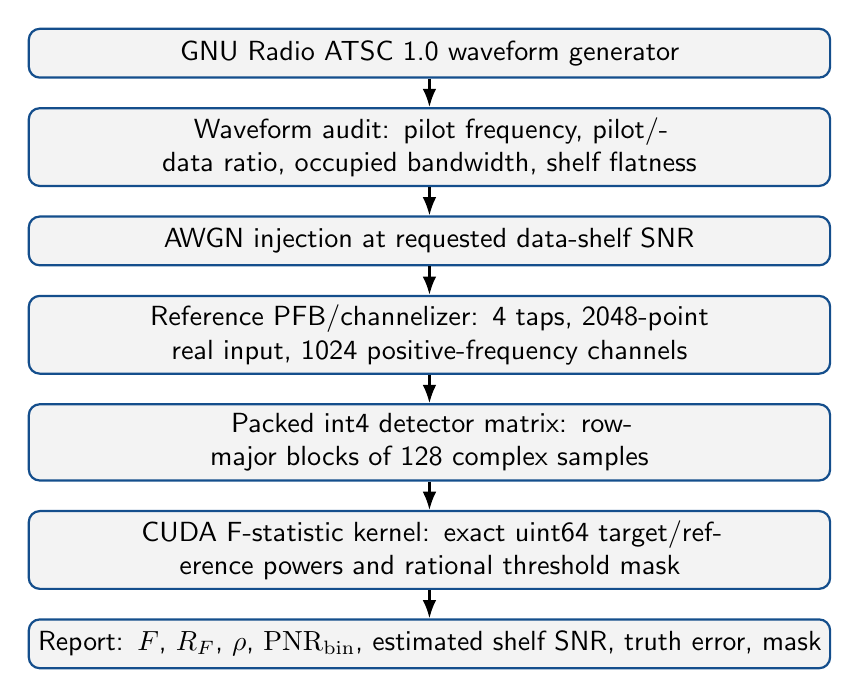
\begin{tikzpicture}[node distance=0.36cm,>=Latex]
\tikzstyle{block}=[rectangle,rounded corners,draw=FStatBlue,thick,fill=LightGray,minimum height=0.62cm,text width=0.82\linewidth,align=center]
\node[block] (a) {GNU Radio ATSC 1.0 waveform generator};
\node[block,below=of a] (b) {Waveform audit: pilot frequency, pilot/data ratio, occupied bandwidth, shelf flatness};
\node[block,below=of b] (c) {AWGN injection at requested data-shelf SNR};
\node[block,below=of c] (d) {Reference PFB/channelizer: 4 taps, 2048-point real input, 1024 positive-frequency channels};
\node[block,below=of d] (e) {Packed int4 detector matrix: row-major blocks of 128 complex samples};
\node[block,below=of e] (f) {CUDA F-statistic kernel: exact uint64 target/reference powers and rational threshold mask};
\node[block,below=of f] (g) {Report: $F$, $R_F$, $\rho$, $\mathrm{PNR}_{\mathrm{bin}}$, estimated shelf SNR, truth error, mask};
\draw[->,thick] (a) -- (b);
\draw[->,thick] (b) -- (c);
\draw[->,thick] (c) -- (d);
\draw[->,thick] (d) -- (e);
\draw[->,thick] (e) -- (f);
\draw[->,thick] (f) -- (g);
\end{tikzpicture}
\caption{Standalone validation flow.  The testbench is self-contained and uses the included reference front end.}
\label{fig:validation_flow}
\end{figure}


\newpage\section{Detection on a Packed Matrix}

Run detection on a prebuilt packed detector matrix:
\begin{lstlisting}[style=shell]
LD_LIBRARY_PATH=/usr/lib/wsl/lib \
PYTHONPATH=src "$HOME/miniconda3/envs/fstat/bin/python" \
  -m pilot_proxy.detect \
  --input-detector-matrix generated/detector_input/detector_matrix_i4.npy \
  --physical-channel 14 \
  --threshold-snr-shelf-db -26
\end{lstlisting}
If \code{detector_matrix_i4.npy} is absent but the batched
\code{detector_blocks_i4.npy} file exists, \code{detect} resolves the default
input to the batched file automatically.  If neither file exists, run
\code{quantize} first.

The detector JSON includes:
\begin{itemize}
  \item \field{selected_weight_layout}
  \item \field{result_schema} with \code{schema_version=pilot_proxy_result_v2}
  \item \field{layout} with \field{frame_size_samples}, \field{num_input_streams}, \field{windows_per_stream}, and \field{detector_rows_per_frame}
  \item \field{threshold_snr_shelf_db}
  \item \field{threshold_pnr_bin_db}
  \item \field{threshold_fstat_raw}
  \item \field{threshold_half_num}
  \item \field{threshold_half_den}
  \item \field{rational_overflow_count}
  \item per-block \field{mask}, powers, F-statistic values, and estimated shelf SNR.
\end{itemize}

\section{Receiver Integration Contract}

The standalone package does not encode telescope-specific assumptions.  Receiver
integrations provide JSON metadata and arrays:
\begin{itemize}
  \item \code{configs/detector_core/pilotproxy_cuda_fstat_v1.json} describes the locked CUDA kernel contract.
  \item \code{receiver_profile.json} describes RF band, channelizer geometry, spectral sense, frame size, input streams, quantization defaults, bin ENBW, and pilot-capture efficiency.
  \item \code{stream_map.json} maps stream indices to feed, polarization, beam, or other receiver-specific identifiers.
  \item Runtime commands such as \code{detect}, \code{evaluate-snr}, and \code{chime-run} bind those metadata files to concrete input arrays and output products.
\end{itemize}

Useful metadata checks:
\begin{lstlisting}[style=shell]
PYTHONPATH=src python -m pilot_proxy.cli check-profile \
  --receiver-profile configs/receiver_profiles/reference_800mhz_pfb.json

PYTHONPATH=src python -m pilot_proxy.cli check-layout \
  --receiver-profile configs/receiver_profiles/chime_dtv_fengine.json \
  --stream-map configs/stream_maps/chime_feed_pol_example.json
\end{lstlisting}

Generate receiver-profile-backed weights with:
\begin{lstlisting}[style=shell]
PYTHONPATH=src python -m pilot_proxy.cli make-weights \
  --receiver-profile configs/receiver_profiles/chime_dtv_fengine.json \
  --detector-core-profile configs/detector_core/pilotproxy_cuda_fstat_v1.json \
  --physical-channel-range 14:36 \
  --weight-coordinate-system post_spectral_sense_normalization \
  --output weights/chime_dtv_weights_k128.bin
\end{lstlisting}

The CHIME profile and stream map are examples requiring data-product
verification.  They are not required by the standalone ATSC/DTV testbench.  The
example stream map contains all 2048 feed-polarization entries so layout checks
exercise the same row-count contract expected by a telescope adapter.

\section{Thresholds}

Users provide \code{threshold_snr_shelf_db}.  Host code converts it to a rational half-threshold.  The kernel then evaluates only integer powers and integer threshold terms.


\begin{figure}[H]
\centering
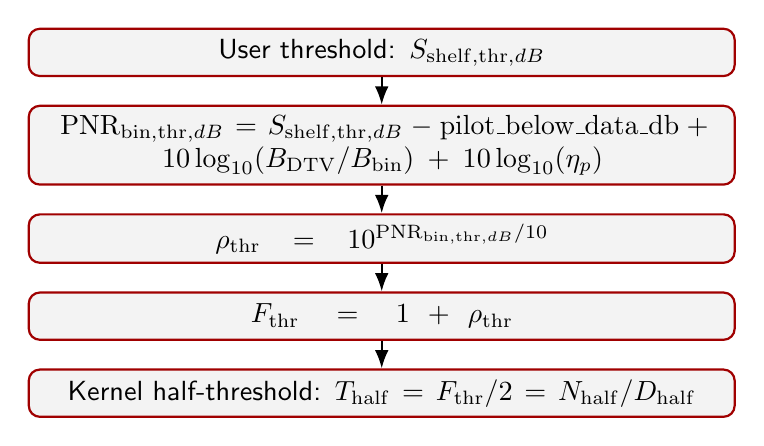
\begin{tikzpicture}[node distance=0.35cm,>=Latex]
\tikzstyle{block}=[rectangle,rounded corners,draw=FStatRed,thick,fill=LightGray,minimum height=0.60cm,text width=0.72\linewidth,align=center]
\node[block] (a) {User threshold: $S_{\mathrm{shelf,thr},dB}$};
\node[block,below=of a] (b) {$\mathrm{PNR}_{\mathrm{bin,thr},dB}=S_{\mathrm{shelf,thr},dB}-\mathrm{pilot\_below\_data\_db}+10\log_{10}(B_{\mathrm{DTV}}/B_{\mathrm{bin}})+10\log_{10}(\eta_p)$};
\node[block,below=of b] (c) {$\rho_{\mathrm{thr}}=10^{\mathrm{PNR}_{\mathrm{bin,thr},dB}/10}$};
\node[block,below=of c] (d) {$F_{\mathrm{thr}}=1+\rho_{\mathrm{thr}}$};
\node[block,below=of d] (e) {Kernel half-threshold: $T_{\mathrm{half}}=F_{\mathrm{thr}}/2=N_{\mathrm{half}}/D_{\mathrm{half}}$};
\draw[->,thick] (a) -- (b);
\draw[->,thick] (b) -- (c);
\draw[->,thick] (c) -- (d);
\draw[->,thick] (d) -- (e);
\end{tikzpicture}
\caption{Threshold coordinate conversion.  The user gives a shelf-SNR threshold; the kernel receives only a fixed-point rational half-threshold.}
\label{fig:threshold_conversion}
\end{figure}


For \(-26\dB\) shelf SNR with the included reference geometry:
\begin{lstlisting}[style=shell]
threshold_snr_shelf_db       = -26.000
threshold_pnr_bin_db         =  -4.364
threshold_pilot_excess_linear=   0.3661
threshold_fstat_raw          =   1.3661
threshold_half_float         =   0.68305
\end{lstlisting}

\section{Standard and Calibrated Conversion}

Standard mode uses:
\begin{lstlisting}[style=shell]
--pilot-below-data-db 11.3
--bin-enbw-hz 3051.7578125
--pilot-capture-efficiency 1.0
--dtv-bandwidth-hz 6000000
\end{lstlisting}
The positive field \field{pilot_below_data_db} means that the pilot power is below the average data-shelf power by that many dB.  If a waveform audit reports \field{measured_pilot_to_data_power_db=-11.9}, then the corresponding positive magnitude is \field{measured_pilot_below_data_db=11.9}.

Use calibrated mode only when external calibration supports the overrides:
\begin{lstlisting}[style=shell]
--pilot-below-data-db VALUE
--bin-enbw-hz VALUE
--pilot-capture-efficiency VALUE
\end{lstlisting}
Every validation report records the values used.

\section{C API Overview}

The public C API is in \code{cuda/f_statistic.h}.  The production path is:
\begin{lstlisting}[style=cstyle,language=C]
int K, N, bits, ref_offset;
FStat_GetSpecs(&K, &N, &bits, &ref_offset);

void* h = FStat_Create(d_in, NULL, detector_rows_per_block);
FStat_Compute_NumDen_Mask_RationalHalf_WithOverflowCount(
    h,
    host_weights,
    threshold_half_num,
    threshold_half_den,
    d_num_out,
    d_den_out,
    d_mask_out,
    d_overflow_count);
FStat_Destroy(h);
\end{lstlisting}
The returned values are:
\begin{equation}
  \mathrm{d\_num\_out}=P_t,\qquad \mathrm{d\_den\_out}=P_{r1}+P_{r2}.
\end{equation}
Use:
\begin{equation}
  F=\frac{2\,\mathrm{num}}{\mathrm{den}}.
\end{equation}
A zero denominator is an invalid reference floor.  The kernel forces the mask to zero.  The C and Python helper routines map zero-denominator pilot excess to zero unless a checked helper is used.

\section{JSON Output Policy}

All JSON reports are strict JSON.  Invalid floating-point values such as NaN or infinity are serialized as \code{null}.  CSV reports may retain NaN text where appropriate for analysis tools.

Every public JSON report includes \field{result_schema} with \code{schema_version=pilot_proxy_result_v2}.  This object records the statistic definitions, layout metadata, calibration constants, threshold conversion, fixed-point contract, and mask convention.

The combined-row statistic is:
\begin{equation}
F = \frac{2\sum_r P_{t,r}}{\sum_r P_{r1,r}+\sum_r P_{r2,r}},
\end{equation}
where \(r\) indexes detector rows.  The rule is to sum powers first, then form \(F\); do not average per-row F-statistics.

The generic mask convention is exclusion, not zero-fill:
\begin{equation}
\bar{P}_{\mathrm{after}} =
\frac{\sum_b P_b(1-M_b)}{\sum_b (1-M_b)}.
\end{equation}
Here \(M_b=1\) means masked/excluded.

\section{Result Summaries}

Use the generic summary helper for compact CSV/JSON statistics:
\begin{lstlisting}[style=shell]
PYTHONPATH=src python -m pilot_proxy.cli summarize-results \
  --input generated/dtv_snr_eval/dtv_snr_eval.json \
  --output-dir generated/summary
\end{lstlisting}
This writes \code{summary.csv} and \code{summary.json}.  Histogram PNGs are
skipped automatically for SNR sweeps because a sweep mixes different
requested-SNR populations.  Histograms are meaningful for fixed-SNR multi-trial
runs, or can be forced explicitly with \code{--histograms always} for
diagnostic work.

\section{Known Limitations}

\begin{itemize}
  \item v0.1.0 is standalone GNU Radio ATSC validation only.
  \item No CHIME/baseband file reader is included.
  \item No telescope-specific stream map is validated beyond example JSON metadata.
  \item No operational threshold is derived from real telescope null statistics.
  \item Receiver profiles are an integration contract, not a validated telescope pipeline.
  \item Wheel-style installation with packaged CUDA and weight resources is not the primary supported mode.
\end{itemize}

\section{Troubleshooting}

\subsection{GNU Radio imports fail}
Use the system GNU Radio Python, typically \code{/usr/bin/python3}, and set \code{PYTHONNOUSERSITE=1}.

\subsection{CUDA shared library not found}
Run \code{make build-kernel SM=<target>} and ensure \code{LD_LIBRARY_PATH} includes the CUDA driver path.  On WSL, use \code{/usr/lib/wsl/lib} and prefer the staged cache copy under \code{~/.cache/pilot_proxy/}.

\subsection{Wrong detector matrix shape}
The packed detector matrix must have dtype \code{int8} and last dimension 128.  Use \code{pilot_proxy.testbench.quantize} to build the expected format.

\subsection{No weights for channel}
The shipped bank covers physical channels 14-36.  Use \code{pilot-proxy list-channels} to list available targets.

\subsection{PNR is null}
If \(F\leq1\), the pilot-excess ratio is non-positive, and \(10\log_{10}(F-1)\) is undefined.  This is expected for noise-only or below-threshold trials.

\begin{thebibliography}{9}
\bibitem{atsc_a53_part2_2011} Advanced Television Systems Committee, \emph{ATSC Digital Television Standard, Part 2: RF/Transmission System Characteristics}, A/53 Part 2:2011, 15 December 2011. \url{https://www.atsc.org/wp-content/uploads/2021/04/A53-Part-2-2011.pdf}
\bibitem{ecfr_73603} Electronic Code of Federal Regulations, 47 CFR \S 73.603, \emph{Numerical designation of television channels}. \url{https://www.ecfr.gov/current/title-47/chapter-I/subchapter-C/part-73/subpart-E/section-73.603}
\bibitem{gnuradio_dtv} GNU Radio Manual, \emph{DTV/ATSC module documentation}. \url{https://www.gnuradio.org/doc/sphinx-3.7.7.1/atsc/index.html}
\bibitem{gnuradio_noise} GNU Radio Manual, \emph{gr::analog::noise\_source}, complex noise-source amplitude convention. \url{https://www.gnuradio.org/doc/doxygen/classgr_1_1analog_1_1noise__source.html}
\end{thebibliography}

\end{document}
